\section{Data heterogeneity}
\label{sec:application}	

\begin{figure}[t]
	\centering
	\begin{minipage}{0.48\linewidth}
		\centering
   		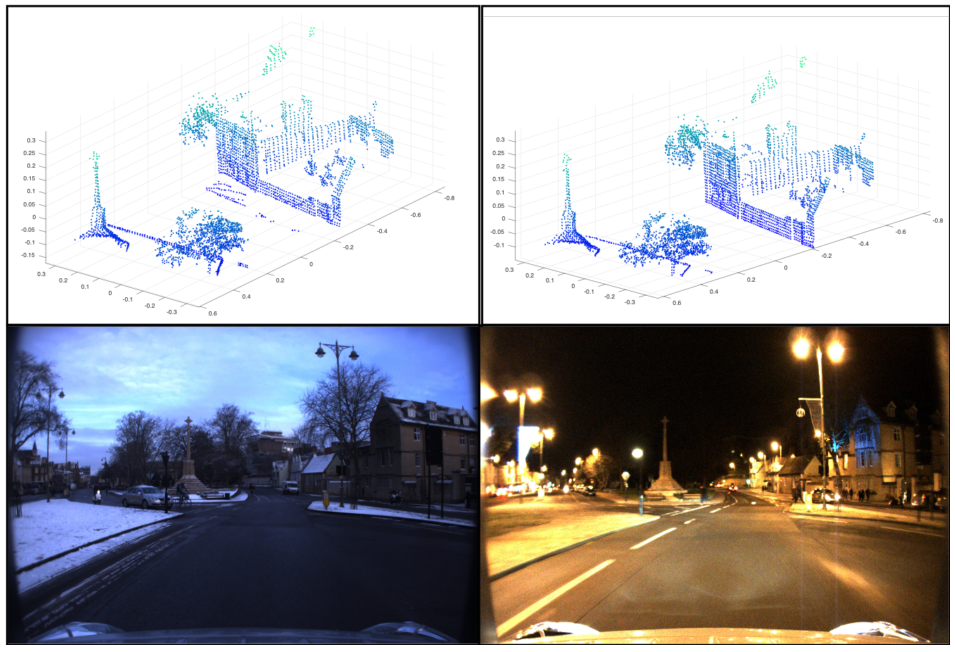
\includegraphics[width=\linewidth]{data_hetero/pointnetvlad.png}
	   		
   		\noindent\rule{\linewidth}{0.4pt}
   		   		
   		\subfigure[][Geometric information]{\label{fig:3d_info}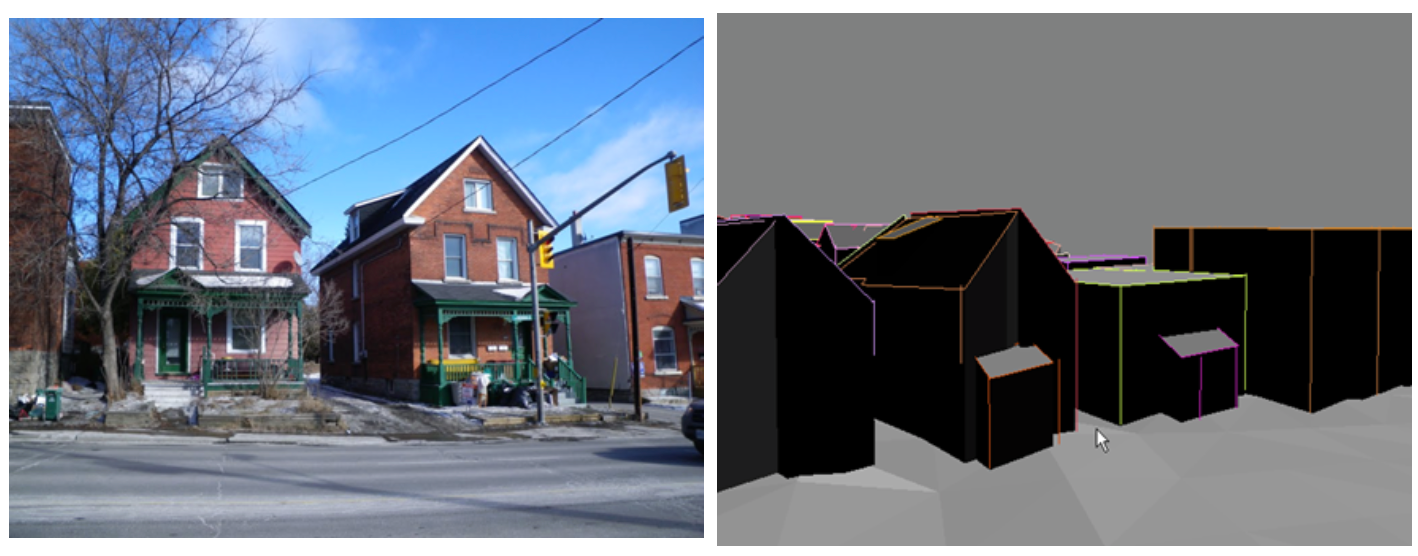
\includegraphics[width=\linewidth]{data_hetero/image_to_DEM.png}}
	\end{minipage}
	\begin{minipage}{0.48\linewidth}
		\centering
   		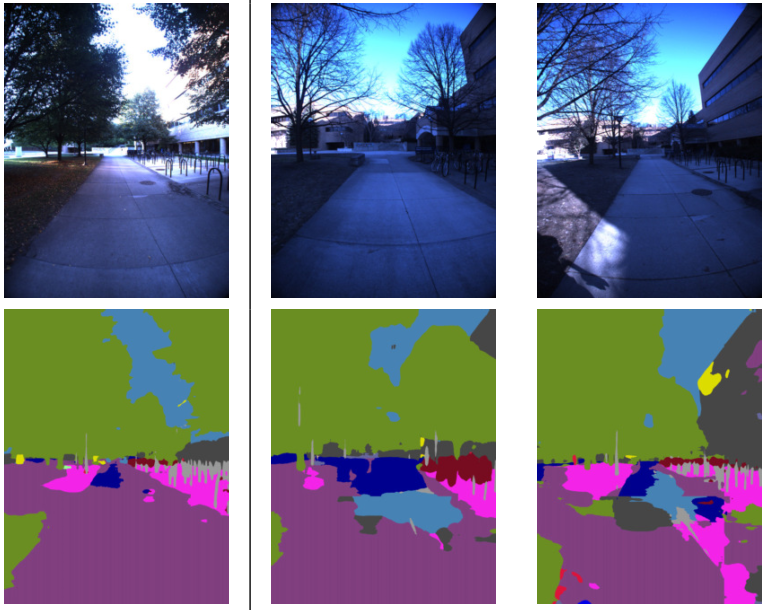
\includegraphics[width=0.95\linewidth]{data_hetero/semantic_vbl.png}
   		
		\noindent\rule{\linewidth}{0.4pt}		
		
   		\subfigure[][Semantic information]{\label{fig:seg_ifo}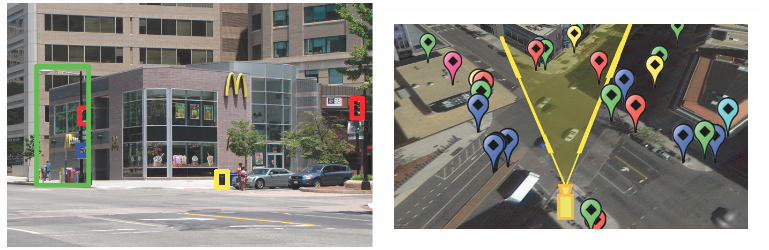
\includegraphics[width=\linewidth]{data_hetero/semantic.png}}
	\end{minipage}
	\caption[Illustration of the data heterogeneity in \ac{vbl}]{\textbf{Illustration of the data heterogeneity in \ac{vbl}:} \ref{fig:3d_info}~From top to bottom: PointNetVLAD~\citep{Uy2018} used to match point cloud for \acs{vbl} and localization system built upon a DEM~\citep{Matei2013}. \ref{fig:seg_ifo}~From top to bottom: data segmentation to help queries (right) to database (left) visual association ~\citep{Schonberger2017a} and localization system with semantic information gathered from OpenStreetMap annotation {Ardeshir2014}. \label{fig:data_div}}
\end{figure}

	Originally, images were the dedicated data to \ac{vbl} system~\citep{Robertson2004}. Still, conventional images for the task of localization have limitations, as mentioned in the previous section (see Section~\ref{sec:changing_environment}). The use of other type of data, such as geometric and semantic information, can circumvent these limitations. This section aims to exhaustively present the three different kinds of data used in \ac{vbl}: optical, geometric and semantic.

	\subsection{Optical information}
		\label{subsec:visual_info}
		\citet{Robertson2004} present the first \ac{vbl} method based on a geo-referenced database of images. Authors work aimed to localize buildings facades; therefore this database reflects the end-user application and was composed of images of front facing buildings. However, depending on the targeted application, the appearance of the database is likely to change. Figure~\ref{fig:visual_info} illustrates the diversity of imagery used for~\ac{vbl}.
		
		\paragraph{Application}
			Most of the \ac{vbl} systems are designed to retrieve the location of a camera within an urban environment, where a GPS signal cannot be properly received. Urban \ac{vbl} systems are categorized in four classes: indoor \ac{vbl}~\citep{Liang2013}, \ac{vbl} for pedestrians (or robots~\citep{Garcia-Fidalgo2015}) inside a city \citep{Robertson2004,Schindler2007,Chen2011,Zhang2006}, vehicles \ac{vbl} on road traffic scenes for urban or suburban navigation~\citep{McManus2014,Milford2015,Qu2016,Brubaker2016} and aerial vehicles localization system~\citep{Wan2016}. The appearance of the images present in the database changes drastically giving the purpose of the visual localization system.
		
		\paragraph{Coverage}			
			By definition, the previously described applications do not cover the same area. For instance, a system design for car pose estimation should be able to localize a vehicle in a larger area than a pedestrian \ac{vbl} system should do. Thus, there exists systems designed for world-wide localization estimation~\citep{Hays2008,Weyand2016,Vo2017} as well as more spatially focused system~\citep{Song2016}. Database coverage can be extended by using wide angle or omnidirectional cameras. Works presented in~\citep{Arandjelovic2016,Iscen2017,Kumar2016mastersThesis,Ramalingam2010,Torii2011,Zamir2010,Zamir2014} use databases composed of spherical panoramas. On the other hand, aerial images are likely to cover large area but restrict \ac{vbl} applications~\citep{Wan2016}.
			
		\paragraph{Database Consistency}
			\label{para:data_consistency}
			Regardless of the type of images used, we distinguish between two kinds of databases: homogeneous and heterogeneous. Homogeneous databases are composed of images gathered through the same optical acquisition system in a restricted time interval. Google street view\footnote{https://www.google.fr/intl/usa/streetview/} or \textit{IGN St\'er\'eopolis} platform~\citep{Paparoditis2012} give access to this kind of database. Homogeneous databases are suitable for applications that perform systematic processing on the data~\citep{Majdik2013,Torii2015}. Conversely, heterogeneous databases are made of images collected by various people with different cameras at inconsistent periods. These databases are often constructed through on-line collaborative platforms, like flickr\footnote{https://www.flickr.com/}, by downloading images associated to specific tags. Heterogeneous databases have the advantage of introducing visual variations in the \ac{vbl} system and therefore improves robustness to appearance changes~\citep{Radenovic2016,Gordo2016} (see Section~\ref{sec:changing_environment}). Additionally, heterogeneous databases are easier to augment or update compared to homogeneous ones.
			
	\subsection{Geometric information}
		\label{subsec:geometric_info}
		As presented in the outlines of this section, adding geometric information aims to overcome the limitations of only-based-optical \ac{vbl}.
        
		\paragraph{Weak Geometry}
			\label{subsubsec:weak_geometry}			
			In \citep{Torii2015,Chen2011}, authors introduce weak geometric clues that describe principal 3D planes present in the scene. This information is then used to modify existing images in the database: for rectification purpose~\citep{Chen2011} or to generate more images in order to cover a larger area~\citep{Torii2015}. \citet{Cham2010} use a 2D buildings outline map for \ac{vbl}. From a given image, authors extract buildings corner and match them according to the map. Along the same line, \ac{vbl} method from~\citep{Arth2015} relies on a 2.5D map of Gratz (schematic buildings outlines boxes from OpenStreetMap\footnote{https://www.openstreetmap.org}). 2D map is also used as geo-reference in the work from~\citep{Brubaker2013} (extended version in~\citep{Brubaker2016}) where authors produce, thanks to a stereo-camera, a path of a vehicle that is afterwards matched against the map. The matching process is embedded in a probabilistic framework to handle large environment. \citet{Baatz2012} introduce the use of a \ac{dem} to perform localization in mountainous terrain~\citep{Ramalingam2010,Tzeng2013,Chen2015}. \citet{Bansal2014} extend this idea in urban localization to perform purely geometric \ac{vbl} with images as query input and \ac{dem} of a city as database. These purely geometric descriptions, also used in~\citep{Matei2013,Christie2016,Ramalingam2010,Ramalingam2011} (see figure~\ref{fig:3d_info}), permit localization independently of the illumination conditions (compared to optically dependant methods, see \S\ref{para:illum}).

		\paragraph{3D geometry}
        \label{subsubsec:3d_geometry}
			Previous section \S\ref{subsec:sfm_methods} emphasizes the growing importance of colourized point clouds obtained by \ac{sfm} in \ac{vbl}. Because such geometric models are built upon images collections, reconstructed point clouds also lie on two categories: homogeneous~\citep{Kendall2015,Kendall2016} and heterogeneous~\citep{Irschara2009,Sattler2011} models (see \S\ref{para:data_consistency}). The addition of geometric relation by \ac{sfm} improves retrieval performances~\citep{Sattler2012a} and permits precise pose estimation of the query, on the contrary of methods based on vanilla images collections.

			However, \ac{sfm} reconstruction is a costly operation. Rather than preprocessing the visual data to recover the geometry of the scene, appropriate sensors permit a direct capture of a 3D scene (\textit{e.g.} stereo camera, depth camera, laser, lidar, etc.). Raw data from depth sensor are often used to add supplementary information channel to the \ac{vbl} system. Works from~\citep{Ni2009,McManus2014,Wan2014} use disparity map from stereo camera. Several authors~\citep{Shotton2013,Guzman-rivera2014,Glocker2015} used active depth camera that project infra-red pattern to estimate depth. Similar technology is used in~\citep{Li2016a} to perform \ac{vbl} in complete obscurity. Consistent 3D models are also used to perform \ac{vbl} task. For indoor localization, works from \citep{Shotton2013,Pascoe2015} use textured model reconstructed from RGB-D sensor~\citep{Shotton2013} or hand-crafted with dedicated software~\citep{Pascoe2015}. City-scale models are used by \citep{Aubry2014,Poglitsch2015,Pascoe2015a,Pascoe2015b,Caselitz2016} to perform outdoor \ac{vbl}. 

\begin{table}[t]
	\centering
	\caption[Data heterogeneity in \ac{vbl}]{\label{tab:data_types}\textbf{Data heterogeneity in \ac{vbl}.} Summary of the various types of data used in \ac{vbl}. First row indicates the type of data present in the database and the first column the type of the query confronted to this database. References in \textbf{bold} denote works using semantic interpretation of the data (see \S\ref{subsec:semantic_info}). $^{\dagger}$~Image-retrieval based methods that compare a input image to a set of images. Numerous references not displayed to readability reason. $^{\ddagger}$~Several works consider \ac{vbl} with as an input a set of images from the same scene rather than only one image input.}

	\renewcommand{\arraystretch}{1.1}
	\newcolumntype{M}[1]{>{\centering\arraybackslash}m{#1}}
	\footnotesize{
	\begin{tabular}{|m{0.13\textwidth} || M{0.18\textwidth} | M{0.18\textwidth} | M{0.18\textwidth} | M{0.18\textwidth} |}
          \hhline{-||----}
		\hfill \bf Database		& Images collection 				& Weak geometry					& SfM						& 3D model \\
          \bf Query 			& \S\ref{subsec:visual_info}			& \S\ref{subsubsec:weak_geometry}		& \S\ref{subsec:sfm_methods} 	& \S\ref{subsubsec:3d_geometry} \\
          \hhline{=::=:=:=:=:}
          Image				& Similarity search$^{\dagger}$ \textbf{\citep{Arandjelovic2014a,Garg2017,Mousavian2015,torralba2003context,Ni2009,Weyand2016}} 		& \citep{Baatz2012,Cham2010,Chen2011,Torii2015} \textbf{\citep{Atanasov2016,Ardeshir2014,Arth2015,Castaldo2015,Wang2015}} &  \citep{Arth2009,Donoser2014,Heisterklaus2014,Irschara2009,Feng2016a,Li2010,Li2012,Lu2015,Lynen2015,Middelberg2014,Sattler2011,Sattler2012,Sattler2015,Sattler2016a,Svarm2014,Zeisl2015}	& \citep{Aubry2014,Mason2011,Russell2011} \\
            \hhline{-||-|-|-|-|}
            Several images$^{\ddagger}$	& \citep{Weyand2016,Zamir2010}		& \citep{Brubaker2016} & \citep{Kroeger2014}								& \textbf{X} \\
            \hhline{-||-|-|-|-|}
            Image + Depth				& \textbf{X}						& \textbf{\citep{Christie2016}}						& \textbf{X}								& \citep{Cavallari,Gee2012,Glocker2013,Glocker2015,Guzman-rivera2014,Shotton2013,Valentin2015,Sizikova2016} \textbf{\citep{Fernandez-Moral2013,Salas-Moreno2013}}\\
            \hhline{-||-|-|-|-|}
            SfM				& \textbf{X}						& \textbf{X}						& \citep{Middelberg2014} \textbf{\citep{Lu2015}}				& \textbf{X} \\
            \hhline{-||-|-|-|-|}
	\end{tabular}
	}
\end{table}

	\subsection{Semantic information}
		\label{subsec:semantic_info}
		Robustness and precision brought by geometric information has a significant cost in term on data acquisition, processing power and storage needs. Nevertheless, there is a good alternative and discriminant data representation: the semantic information. Semantic representation has received a growing interest in research community~\citep{Liu2016a}, in particular for robot navigation purpose~\citep{Kostavelis2015}. Semantic-based methods are notably efficient to perform robust \ac{vbl} to all kind of appearance changes. Indeed, by capturing a meaningful information about the scene composition, this approach is by definition invariant to local changes in appearance and in geometry. Semantic information used in \ac{vbl} are classified between two classes: segmentation and categorization. Segmentation involves local methods that recognize within a data sub-parts with a semantic meaning (\textit{e.g.} object detection in an image). On the other hand, categorization can be seen as global descriptors that associated semantic labels to a given data (\textit{e.g.} scenes interpretation~\citep{Deng2009}).
		
		\paragraph{Segmentation}
			The world ``semantic'' can be understood in different ways: \citet{Fernandez-Moral2013} semantic approach consists of extracting planar surfaces in a scene, while in~\citep{Salas-Moreno2013} authors segment a point cloud to extract objects with higher semantic meaning, like chair or table. Semantic approaches encode the data with a graph where nodes represent objects (plan in~\citep{Fernandez-Moral2013}, furnitures in~\citep{Salas-Moreno2013}) and edges spatial relations between objects. Graph representation offers a compressed data representation capable to handle local changes and minor measurement errors~\citep{Stumm2015}. Semantic segmentation is used in~\citep{Lu2015} to narrow the search scope and in~\citep{Ardeshir2014,Castaldo2015,Christie2016} to directly recover the pose of the query (illustration on figure~\ref{fig:seg_ifo}). Works described in~\citep{Arandjelovic2014a,Mousavian2015} consider the re-weighting of extracted local features in image according to the semantic class of the pixel obtained by image segmentation. Using this information, authors reduce the influence of local features that are not semantically robust for \ac{vbl}, like vegetation or cars. In a same manner, \citet{Arth2015} present concrete application of semantic segmentation of an image to reinforce hypothesis about building facades segmentation (the image is segmented with a SVM classifier). On the other hand, several methods rely on annotated map~\citep{Atanasov2016,Wang2015} or Geographic Information System (GIS)~\citep{Ardeshir2014,Castaldo2015,Qu2015} to guide the localization.
	    	
		\paragraph{Categorization}
			Scene categorization~\citep{Wu2009} is a different manner to exploit semantic clues for \ac{vbl}. High level semantic features have been popularized with the augmentation of labelled data and the accessibility of high computation power devices (GPU, Cloud Computing). ImageNet challenge introduced in 2009 by~\citep{Deng2009} permits the emergence of fast and robust classification methods, like the one described in~\citep{Krizhevsky2012}. Image classification produces a sub-sample of semantically identical images associated to a class. In \ac{vbl}, classification can be used to decimate the database in order to proceed in a subsequent step to a more precise pose search. This method is successfully applied in~\citep{Sunderhauf2015}, where the used \ac{cnn} has a dual-purpose: narrowing the search scope by semantic labelling and producing a global descriptor by weight aggregation (see \S~\ref{para:global_cnn}). In~\citep{torralba2003context,Ni2009}, classical learning methods like Gaussian Mixture Models (GMM) or epitome are employed for associating images to a finite number of possible locations. Recent work from~\citep{Garg2017} use semantic categorization in order to establish transition probabilities from a given type of environment to another one. Authors embed this framework in the SeqSLAM algorithm, improving the global system accuracy. Finally, works presented in~\citep{Hays2008,Weyand2016} consider the problem of classification of images at a world-wide level.
			
	\subsection{Cross-data localization}
	\label{subsec:cross_data}        
		We have presented in this section three different kinds of information that can be used for \ac{vbl}: optical, geometric and semantic. These types of data are commonly used together to improve localization. In this part, we consider the scenario where all types of data are not available at query time, for instance if the database uses more complete representation of the environment than the query input. It is a common scenario because some data are more difficult to acquire or required specific sensors (\textit{e.g.} geometric information). In this case, methods have to deal with asymmetric representation of the environment in term of data type. We denote this problem cross-data \ac{vbl} and classify the methods founded in the literature in two categories: methods using a common description regardless of the type of data and methods projecting one type of data within another data representation space.
		
    	\paragraph{Common description}
    		Features to Points (F2P) \ac{vbl} (see \S\ref{subsec:sfm_methods}) oppose 2D images to 3D point cloud. In fact, all the features are exclusively extracted from images. On the other hand, semantic abstraction permit cross-data comparison by considering semantic object extracted from various types of data: images to 2D building outline map~\citep{Cham2010}, images to map~\citep{Ardeshir2014,Qu2015,Castaldo2015,Brubaker2016}, RGB-D data to \ac{dem}~\citep{Christie2016}, etc. Referring to a similar physical entity, not necessary semantic, is also a manner to link information from various types of data. Images to DEM correspondences is performed in \citep{Bansal2014} based on a method relying on purely geometric clues extracted both in the image and the model. Recent work from \citep{Sizikova2016,Li2017} use joint descriptors to merge RGB and depth data into a single feature.
					
		\paragraph{Data projection}
			Another widely used method for combining data of different types consists of projecting one of the engaged data into the representation space of the other. For instance, lot of methods consider the challenging problem of registering photographies upon 3D models~\citep{Baatz2012,Kendall2015,Arth2015,Pascoe2015,Pascoe2015a,Pascoe2015b}. Similarity comparison is performed thanks to synthetic images generated from the 3D models \citep{Russell2011,Mason2011,Aubry2014,Poglitsch2015}. Notice the synthesis of skyline profiles from DEM in the work of \citet{Baatz2012}. Special attention is paid to placement of the artificial cameras that generate fake 2D views \citep{Irschara2009,Gee2012,Torii2015}: \citet{Aubry2014} generate cameras over a regular grid to cover a maximal area. A pruning is then applied to only keep the most discriminant views.

To conclude this section, the different types of data used in \ac{vbl} methods are summarized in table~\ref{tab:data_types}.

